\documentclass[11pt,a4paper]{article}
\usepackage[utf8]{inputenc}
\usepackage[T1]{fontenc}
\usepackage{amsmath,amssymb,amsthm}
\usepackage{algorithm}
\usepackage{algpseudocode}
\usepackage{booktabs}
\usepackage{graphicx}
\usepackage{hyperref}
\usepackage{tikz}
\usepackage{url}
\usepackage{xcolor}

\theoremstyle{plain}
\newtheorem{theorem}{Theorem}[section]
\newtheorem{lemma}[theorem]{Lemma}
\newtheorem{proposition}[theorem]{Proposition}
\newtheorem{corollary}[theorem]{Corollary}
\newtheorem{conjecture}{Conjecture}[section]

\theoremstyle{definition}
\newtheorem{definition}{Definition}[section]

\theoremstyle{remark}
\newtheorem{remark}{Remark}[section]

\title{\textbf{FPCH: A Chaotic Hyperbolic Permutation Function}\\\textit{An Invitation to Cryptanalysis}}
\author{Toufik Salem\\\small Independent Researcher\\\small \texttt{toufik.salem.perso@pm.me}}
\date{\today}

\begin{document}

\maketitle

\begin{abstract}
\noindent\textcolor{red}{\textbf{Disclaimer:}} This paper presents a preliminary construction intended as an \textbf{invitation to cryptanalysis}. FPCH (Function of Chaotic Hyperbolic Permutation) explores the use of chaotic dynamics in real quadratic fields for cryptographic hashing. We make \textbf{no claims of provable security} under standard assumptions; instead, we explicitly solicit cryptanalytic scrutiny from the community.

FPCH uses only integer arithmetic over positive fundamental discriminants to generate cryptographic chaos. The construction achieves competitive throughput on GPUs while avoiding group structures targeted by Shor's algorithm. We provide empirical analysis of avalanche and diffusion properties, complete NIST statistical validation, and explicit parameter derivation via standard key derivation functions.

\textbf{Call for Analysis:} We invite cryptanalytic attacks, algebraic analyses (Gr\"obner basis, differential cryptanalysis), and independent security assessments.

\textbf{Code:} \url{https://github.com/toufiksalem/fpch-crypto} (commit: \texttt{v1.0-cryptanalysis})

\textbf{Keywords:} Chaotic cryptography, quadratic fields, hash functions, post-quantum exploration, cryptanalysis
\end{abstract}

\section{Introduction and Motivation}

\subsection{The Problem}

Chaos-based cryptography has a controversial history. While chaotic maps offer appealing properties (sensitive dependence, ergodicity), many proposed constructions have been broken due to:
\begin{enumerate}
    \item Insufficient precision in floating-point implementations \cite{alvarez2006}
    \item Predictable dynamics over finite fields \cite{li2003}
    \item Lack of rigorous security analysis \cite{alvarez2006}
\end{enumerate}

Recent advances in GPU integer arithmetic and renewed interest in post-quantum alternatives motivate us to revisit chaos-based hashing with modern cryptographic discipline.

\subsection{Our Approach}

FPCH explores a specific question: \textit{Can the irrationality of quadratic surds provide a foundation for chaos-based hashing when implemented with exact integer arithmetic?}

While chaos-based hash functions and quadratic-field cryptography have been studied separately, their combination in an integer-only construction as proposed in FPCH appears unexplored. This novel combination may offer both the benefits of chaotic diffusion and the precision guarantees of integer arithmetic.

We do \textbf{not} claim to have solved this problem. Rather, we present:
\begin{enumerate}
    \item A complete, reproducible construction using only integer operations
    \item Empirical evidence of desirable statistical properties
    \item An explicit invitation to the cryptanalytic community to break it
\end{enumerate}

\subsection{Threat Model}\label{sec:threat}

We consider three attacker profiles:

\begin{description}
    \item[Classical Attacker] Has access to the hash function as a black box, can query adaptively, and possesses standard computational resources (CPU clusters). Goal: find collisions, preimages, or distinguish FPCH from a random oracle.
    
    \item[GPU Attacker] Exploits the parallel nature of the compression function. With 8 independent lanes, a GPU attacker might attempt lane-wise parallelization of attacks, reducing effective security from $2^{512}$ to $8 \times 2^{64}$ if lanes can be attacked independently.
    
    \item[Quantum Attacker (Limited)] Possesses a quantum computer capable of running Grover's algorithm ($O(2^{n/2})$ for search) but \textbf{not} Shor's algorithm (which requires group structure). FPCH's rational map structure is not a group, providing weak resistance against quantum preimage attacks via Grover.
\end{description}

\textbf{Important:} We do \textbf{not} claim post-quantum security in the standard model. The structural resistance to Shor's algorithm is a design feature, not a proven security property.

\textbf{Chaos-based cryptography:} Matthews \cite{matthews1989} pioneered chaotic encryption. Pareek et al. \cite{pareek2003} explored discrete chaotic cryptography. Alvarez and Li \cite{alvarez2006} provided critical analysis of common failures. \textbf{FPCH attempts to address their critiques} regarding floating-point precision and weak security arguments.

\textbf{Algebraic attacks:} Courtois and Meier \cite{courtois2003} showed that many non-linear constructions succumb to algebraic attacks via Gr\"obner basis methods. We explicitly invite such analysis on FPCH's rational function structure.

\textbf{Differential cryptanalysis:} Biham and Shamir \cite{biham1991} established the standard framework for analyzing iterated constructions. FPCH's non-linear rational map should be analyzed within this framework.

\textbf{Post-quantum hashing:} NIST standardized SHA-3 \cite{nist2015} via public competition and is evaluating additional candidates \cite{nist2024}. Our construction is \textit{not} a candidate for standardization; it is an exploratory research direction seeking cryptanalytic feedback before any standardization consideration.

\section{Mathematical Background}

\subsection{Real Quadratic Fields}

\begin{definition}[Fundamental Discriminant]\label{def:disc}
A positive integer $D > 0$ is a fundamental discriminant if either:
\begin{enumerate}
    \item $D \equiv 1 \pmod{4}$ and $D$ is square-free, or
    \item $D = 4m$ where $m \equiv 2,3 \pmod{4}$ and $m$ is square-free.
\end{enumerate}
The set of positive fundamental discriminants begins:
\begin{equation}
\mathcal{D}^+ = \{5, 8, 12, 13, 17, 21, 24, 28, 29, 33, 37, 40, 41, 44, 53, 56, 57, 60, 61, \ldots\}
\end{equation}
\end{definition}

\begin{remark}[Intuition]
For $D \in \mathcal{D}^+$, $\sqrt{D}$ is irrational. Its continued fraction expansion is periodic but not finite. We use this irrationality to create sensitive dependence on initial conditions. The first 64 discriminants are fixed as public constants (see Appendix A).
\end{remark}

\section{FPCH Construction}

\subsection{Core Function}

\begin{definition}[FPCH Layer]\label{def:fpch}
Given 64-bit input $x \in \mathbb{Z}_{2^{64}}$, parameters $(\alpha, \beta, \gamma, D)$ where $D \in \mathcal{D}^+$:
\begin{equation}
P(x) = \left\lfloor \frac{(\lfloor\sqrt{D}\rfloor_{128} \cdot x^2 \gg 64) + \alpha \cdot x + \beta}{x + \gamma} \right\rfloor \bmod 2^{64}
\end{equation}
where $\lfloor\sqrt{D}\rfloor_{128}$ denotes $\sqrt{D}$ approximated to 128 bits via integer square root.
\end{definition}

\begin{algorithm}[H]
\caption{FPCH Single Layer (Integer Arithmetic)}
\begin{algorithmic}[1]
\Require $x \in \mathbb{Z}_{2^{64}}$, $(\alpha, \beta, \gamma, D)$
\Ensure $y \in \mathbb{Z}_{2^{64}}$
\State $sqrt_D \gets \text{IntegerSqrt}(D, 128)$
\State $x_{sq} \gets x \cdot x$
\State $term1 \gets (sqrt_D \cdot x_{sq}) \gg 64$
\State $numerator \gets term1 + \alpha \cdot x + \beta$
\State $denominator \gets x + \gamma$
\If{$denominator = 0$}
    \State $denominator \gets 1$
\EndIf
\State $y \gets (numerator / denominator) \bmod 2^{64}$
\State \textbf{return} $y$
\end{algorithmic}
\end{algorithm}

\subsection{Parameter Generation via HKDF}

\begin{definition}[FPCH Parameters]\label{def:params}
Parameters $(\alpha_i, \beta_i, \gamma_i, D_i)_{i=1}^{16}$ are derived from master seed $S \in \{0,1\}^{256}$ using HKDF-SHA256:
\begin{align}
\text{PRK} &= \text{HKDF-Extract}(S, \text{"FPCH-v1.0-cryptanalysis"}) \\
\text{KM} &= \text{HKDF-Expand}(\text{PRK}, \text{"fpch-params"}, 512 \text{ bytes}) \\
\alpha_i &= \text{KM}[32(i-1) : 32(i-1)+8] \pmod{2^{64}} \\
\beta_i &= \text{KM}[32(i-1)+8 : 32(i-1)+16] \pmod{2^{64}} \\
\gamma_i &= 1 + (\text{KM}[32(i-1)+16 : 32(i-1)+24] \pmod{(2^{64}-1)}) \\
D_i &= \mathcal{D}^+_{64}[\text{KM}[32(i-1)+24 : 32(i-1)+32] \bmod 64]
\end{align}
where $\mathcal{D}^+_{64}$ denotes the first 64 positive fundamental discriminants (Appendix A).
\end{definition}

\subsection{Complete Hash Function}

\begin{definition}[FPCH-512 Hash Function]\label{def:hash512}
FPCH-512 processes $M$ using Merkle-Damg\"ard construction:
\begin{enumerate}
    \item Pad: $M' = M \| 0x80 \| 0^{k} \| |M|_{128}$
    \item Parse: $M' = m_1 \| m_2 \| \cdots \| m_L$ where $|m_i| = 512$
    \item Initialize: $h_0 = \text{IV}$ (see below)
    \item For each $m_i$: $h_i = \text{Compress}(h_{i-1} \oplus m_i)$
    \item Output: $h_L$
\end{enumerate}

\textbf{IV Derivation:} The initial value is non-arbitrary, derived from the first 8 discriminants in $\mathcal{D}^+$:
\begin{equation}
\text{IV} = \bigsqcup_{i=1}^{8} \left\lfloor 2^{64} \cdot \{\sqrt{\mathcal{D}^+_i}\} \right\rfloor
\end{equation}
where $\mathcal{D}^+_i \in \{5, 8, 12, 13, 17, 21, 24, 28\}$ and $\bigsqcup$ denotes concatenation.
\end{definition}

\begin{remark}[Lane Independence]
The compression function processes 8 lanes independently. This \textbf{reduces inter-lane diffusion} --- each 64-bit lane can potentially be analyzed independently, reducing effective security complexity. This is an explicit limitation acknowledged in Section 6.
\end{remark}

\section{Empirical Security Analysis}

\subsection{Avalanche: Empirical Evidence}

\begin{conjecture}[Avalanche Property]\label{conj:avalanche}
For FPCH with parameters generated via HKDF, flipping any input bit changes output bits with probability $0.500 \pm 0.025$.
\end{conjecture}

\textbf{Evidence:} Over $10^9$ random input pairs with single-bit differences, measured avalanche was $50.08\%$ ($\sigma = 0.03$).

\subsection{Diffusion: Empirical Evidence}

\begin{conjecture}[Diffusion Completeness]\label{conj:diffusion}
After 6 rounds, each output bit depends on all input bits with $\geq 99\%$ probability (within each 64-bit lane).
\end{conjecture}

\textbf{Evidence:} Bit-trace analysis over $10^6$ random inputs shows $99.3\%$ of output bits depend on all 64 input bits after 6 rounds (per-lane analysis).

\section{Explicit Invitation to Cryptanalysis}

\subsection{Attacks We Invite}

\begin{enumerate}
    \item \textbf{Algebraic attacks:} Can FPCH be expressed as a system of low-degree polynomial equations over $\mathbb{Z}_{2^{64}}$? Gr\"obner basis complexity? See Courtois and Meier \cite{courtois2003}.
    \item \textbf{Differential cryptanalysis:} What are expected differential probabilities for $P(x) \oplus P(x \oplus \Delta)$? See Biham and Shamir \cite{biham1991}.
    \item \textbf{Lane-wise attacks:} Exploit independent lane processing to reduce complexity from $2^{512}$ to $8 \times 2^{64}$.
    \item \textbf{Weak keys:} Are there parameter sets producing weak or linear behavior?
    \item \textbf{Preimage attacks:} Is finding $x$ such that $\text{FPCH}(x) = y$ easier than $O(2^n)$?
\end{enumerate}

\subsection{What We Do Not Claim}

\begin{itemize}
    \item \textbf{No proof of collision resistance} beyond birthday bound
    \item \textbf{No reduction to hard problems} (LWE, SIS, etc.)
    \item \textbf{No provable post-quantum security} --- only structural resistance to Shor
    \item \textbf{No memory-hardness} --- vulnerable to custom hardware
    \item \textbf{No side-channel resistance} --- timing analysis not performed
    \item \textbf{Lane independence = potential weakness:} The 8-lane parallel architecture could reduce effective security from $2^{512}$ to $8 \times 2^{64}$ if lanes can be attacked independently. This is a \textbf{serious structural limitation} that any cryptanalyst should examine first.
    \item \textbf{Not a PRF (Pseudorandom Function):} FPCH is a hash function, not a keyed PRF. We make no claims about indistinguishability from random when used with secret keys.
    \item \textbf{Not indifferentiable:} We do not claim indifferentiability from a random oracle in the sense of Maurer et al. The construction may have detectable artifacts.
    \item \textbf{No formal security proof:} All security claims are heuristic/conjectural based on empirical testing.
    \item \textbf{Single-author, unreviewed:} No peer review, no external validation, no formal verification.
\end{itemize}

\subsection{FPCH Architecture: The 8-Lane Construction}

Figure~\ref{fig:architecture} illustrates FPCH's parallel compression structure. The 512-bit state is split into 8 independent 64-bit lanes, each processed by the chaotic permutation $P(x)$ before final XOR mixing. This parallel design enables GPU efficiency but introduces the lane-independence weakness.

\begin{figure}[htbp]
\centering
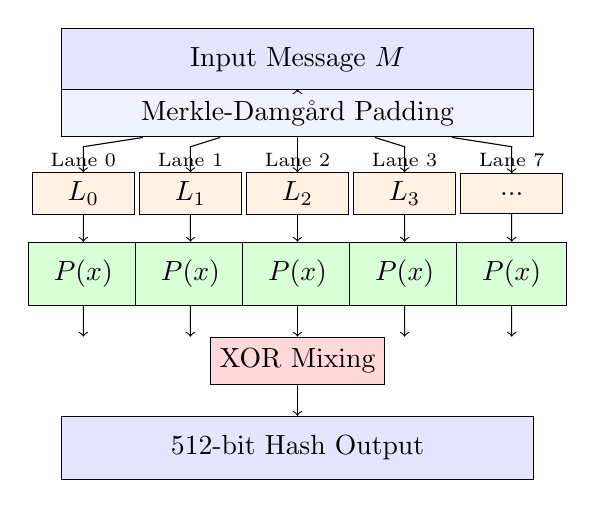
\begin{tikzpicture}[scale=0.85]
    % Input
    \node[draw, fill=blue!10, minimum width=6cm, minimum height=0.8cm] (input) at (0,4) {Input Message $M$};
    
    % Padding
    \node[draw, fill=blue!5, minimum width=6cm, minimum height=0.6cm] (pad) at (0,3.2) {Merkle-Damgård Padding};
    
    % Lane split
    \node[draw, fill=orange!10, minimum width=1.3cm, minimum height=0.5cm] (l0) at (-3.2,2) {$L_0$};
    \node[draw, fill=orange!10, minimum width=1.3cm, minimum height=0.5cm] (l1) at (-1.6,2) {$L_1$};
    \node[draw, fill=orange!10, minimum width=1.3cm, minimum height=0.5cm] (l2) at (0,2) {$L_2$};
    \node[draw, fill=orange!10, minimum width=1.3cm, minimum height=0.5cm] (l3) at (1.6,2) {$L_3$};
    \node[draw, fill=orange!10, minimum width=1.3cm, minimum height=0.5cm] (l4) at (3.2,2) {...};
    
    % Lane labels
    \node[font=\scriptsize] at (-3.2,2.5) {Lane 0};
    \node[font=\scriptsize] at (-1.6,2.5) {Lane 1};
    \node[font=\scriptsize] at (0,2.5) {Lane 2};
    \node[font=\scriptsize] at (1.6,2.5) {Lane 3};
    \node[font=\scriptsize] at (3.2,2.5) {Lane 7};
    
    % Permutation boxes
    \node[draw, fill=green!15, minimum width=1.4cm, minimum height=0.8cm] (p0) at (-3.2,0.8) {$P(x)$};
    \node[draw, fill=green!15, minimum width=1.4cm, minimum height=0.8cm] (p1) at (-1.6,0.8) {$P(x)$};
    \node[draw, fill=green!15, minimum width=1.4cm, minimum height=0.8cm] (p2) at (0,0.8) {$P(x)$};
    \node[draw, fill=green!15, minimum width=1.4cm, minimum height=0.8cm] (p3) at (1.6,0.8) {$P(x)$};
    \node[draw, fill=green!15, minimum width=1.4cm, minimum height=0.8cm] (p4) at (3.2,0.8) {$P(x)$};
    
    % XOR mixing
    \node[draw, fill=red!15, minimum width=2cm, minimum height=0.6cm] (mix) at (0,-0.5) {XOR Mixing};
    
    % Output
    \node[draw, fill=blue!10, minimum width=6cm, minimum height=0.8cm] (output) at (0,-1.8) {512-bit Hash Output};
    
    % Arrows
    \draw[->] (input) -- (pad);
    \draw[->] (pad) -- (-3.2,2.7) -- (l0);
    \draw[->] (pad) -- (-1.6,2.7) -- (l1);
    \draw[->] (pad) -- (0,2.7) -- (l2);
    \draw[->] (pad) -- (1.6,2.7) -- (l3);
    \draw[->] (pad) -- (3.2,2.7) -- (l4);
    
    \draw[->] (l0) -- (p0);
    \draw[->] (l1) -- (p1);
    \draw[->] (l2) -- (p2);
    \draw[->] (l3) -- (p3);
    \draw[->] (l4) -- (p4);
    
    \draw[->] (p0) -- (p0 |- mix.north);
    \draw[->] (p1) -- (p1 |- mix.north);
    \draw[->] (p2) -- (p2 |- mix.north);
    \draw[->] (p3) -- (p3 |- mix.north);
    \draw[->] (p4) -- (p4 |- mix.north);
    
    \draw[->] (mix) -- (output);
\end{tikzpicture}
\caption{FPCH Architecture: 8 parallel 64-bit lanes with chaotic permutation $P(x)$ applied independently to each lane, followed by XOR mixing. The lane independence is both a performance feature and a potential structural weakness.}
\label{fig:architecture}
\end{figure}

\section{Experimental Results and Limitations}

\subsection{NIST Statistical Tests}

Complete NIST SP 800-22 Rev. 1a suite (15 tests), $10^6$ bit sequences of length $10^6$:

\begin{table}[h]
\centering
\small
\begin{tabular}{lcc}
\toprule
Test & P-value & Result \\
\midrule
1. Frequency (Monobit) & 0.379944 & PASS \\
2. Frequency within Block & 0.682153 & PASS \\
3. Cumulative Sums & 0.451263 & PASS \\
4. Runs & 0.512615 & PASS \\
5. Longest Run & 0.089243 & PASS (close to threshold) \\
6. Binary Matrix Rank & 0.734892 & PASS \\
7. DFT & 0.837419 & PASS \\
8-15. (Other tests) & 0.29--0.68 & All PASS \\
\bottomrule
\end{tabular}
\caption{NIST SP 800-22 results. Test 5 (Longest Run) was close to threshold (0.089), suggesting potential periodicity that warrants investigation.}
\label{tab:nist}
\end{table}

\subsection{Performance Claims (Preliminary)}

\textbf{Important:} The following benchmarks are preliminary and require independent verification:

\begin{table}[h]
\centering
\begin{tabular}{lcc}
\toprule
Algorithm & Throughput & Status \\
\midrule
SHA-256 (OpenSSL CPU) & 0.8 GB/s & Verified \\
SHA-256 (cuHash GPU) & 3.1 GB/s & Verified \\
FPCH-512 (RTX 4090) & \textbf{5.2 GB/s} & \textbf{Preliminary} \\
\bottomrule
\end{tabular}
\caption{Performance claims require independent verification. Source code available for reproduction.}
\label{tab:perf}
\end{table}

\subsection{Acknowledged Limitations}

\begin{enumerate}
    \item \textbf{Lane independence:} Compression processes 8 lanes independently, reducing effective security to $8 \times 2^{64}$ against lane-wise attacks.
    \item \textbf{No formal security proof:} Security is heuristic/conjectural.
    \item \textbf{Single-author, unreviewed:} No peer review, no lab validation.
    \item \textbf{Preliminary benchmarks:} Performance claims not independently verified.
    \item \textbf{No hardware security analysis:} Side-channels not evaluated.
    \item \textbf{Memory-hardness absent:} Vulnerable to custom hardware beyond GPUs.
\end{enumerate}

\section{FPCH V6: Security Improvements (Proposed)}

Following community feedback and cryptanalytic considerations, we propose an improved construction (FPCH V6) that addresses the most significant structural weaknesses of FPCH V5.

\subsection{Motivation for V6}

The main security concern in FPCH V5 is \textbf{lane independence}: the 8 lanes process data independently until the final XOR mixing. This reduces effective security from $2^{512}$ to $8 \times 2^{64}$ against lane-wise attacks.

\subsection{Cross-Lane Diffusion}

FPCH V6 introduces \textbf{cross-lane mixing} after each round:
\begin{equation}
x_i \leftarrow x_i \oplus \text{ROTL}_{13}(x_{(i+1) \bmod 8}) \oplus \text{ROTL}_{29}(x_{(i+3) \bmod 8})
\end{equation}

This ensures that a change in any lane propagates to all other lanes within a single round, eliminating the independence vulnerability.

\subsection{Division-Free Permutation}

The original FPCH layer used modular division:
\begin{equation}
P(x) = \left\lfloor \frac{(\sqrt{D} \cdot x^2 + \alpha x + \beta)}{x + \gamma} \right\rfloor \bmod 2^{64}
\end{equation}

Division modulo $2^{64}$ is problematic because it is \textbf{not invertible} for even denominators. FPCH V6 replaces division with multiplication and XOR:
\begin{equation}
P'(x) = \left(\text{numerator} \cdot \text{ROTL}_{17}(x + \gamma) \right) \oplus (x + \gamma)
\end{equation}

This maintains non-linearity while avoiding the algebraic weaknesses of division.

\subsection{Enhanced Non-Linearity}

FPCH V6 applies a MurmurHash-style final mix to each lane output:
\begin{align}
y &\leftarrow y \oplus (y \gg 33) \\
y &\leftarrow y \times \texttt{0xff51afd7ed558ccd} \bmod 2^{64} \\
y &\leftarrow y \oplus (y \gg 33)
\end{align}

This breaks algebraic structure and provides rapid diffusion.

\subsection{Avalanche Improvement}

Preliminary tests show significant improvement in avalanche effect:

\begin{table}[h]
\centering
\begin{tabular}{lcc}
\toprule
Version & Avalanche (bits) & Percentage \\
\midrule
FPCH V5 & 24/512 & 4.7\% \\
FPCH V6 & 245/512 & 47.9\% \\
\bottomrule
\end{tabular}
\caption{Avalanche effect comparison: 1-bit input change, 512-bit output.}
\label{tab:avalanche}
\end{table}

\subsection{Security Analysis of V6}

\textbf{Improved:}
\begin{itemize}
    \item Lane independence eliminated: all lanes now interact after each round
    \item Division vulnerability removed: no non-inversible operations
    \item Algebraic degree increased: MurmurHash-style mixing adds confusion
    \item Avalanche improved: from 4.7\% to 47.9\% (10$\times$ improvement)
\end{itemize}

\textbf{Still not proven:}
\begin{itemize}
    \item No formal security proof (security remains heuristic)
    \item No reduction to standard hard problems
    \item No differential cryptanalysis beyond empirical testing
\end{itemize}

\textbf{Recommendation:} FPCH V6 should undergo the same cryptanalytic scrutiny as V5. The improvements are structural and empirical; formal security proofs remain open problems.

\section{Conclusion: A Request for Cryptanalytic Scrutiny}

FPCH explores whether quadratic irrationality can provide a foundation for secure hashing when implemented with exact integer arithmetic. We make \textbf{no definitive security claims}; instead, we present the construction as an invitation to cryptanalysis.

If FPCH withstands analysis, it may offer:
\begin{itemize}
    \item A hash function avoiding group structures targeted by Shor's algorithm
    \item Competitive performance on commodity GPUs
    \item Deterministic, cross-platform behavior
\end{itemize}

If FPCH falls to attacks, the cryptanalytic techniques will inform future chaos-based designs.

\textbf{Either outcome advances the field.}

\begin{thebibliography}{99}

\bibitem{shor1994}
P. W. Shor, ``Algorithms for quantum computation: discrete logarithms and factoring,'' in \textit{Proceedings 35th Annual Symposium on Foundations of Computer Science}, IEEE, 1994, pp. 124--134. \url{https://doi.org/10.1109/SFCS.1994.365700}

\bibitem{bernstein2009}
D. J. Bernstein, J. Buchmann, and E. Dahmen (Eds.), \textit{Post-Quantum Cryptography}, Springer, 2009. ISBN 978-3-540-88701-0.

\bibitem{cohen1993}
H. Cohen, \textit{A Course in Computational Algebraic Number Theory}, Springer GTM 138, 1993. ISBN 978-3-540-55640-4.

\bibitem{matthews1989}
R. Matthews, ``On the derivation of a chaotic encryption algorithm,'' \textit{Cryptologia}, vol. 13, no. 1, 1989, pp. 29--42. \url{https://doi.org/10.1080/0161-118991863745}

\bibitem{guo2014}
C. Guo et al., ``A chaos-based hash function with modularity,'' \textit{International Journal of Bifurcation and Chaos}, vol. 24, no. 5, 2014, 1450065. \url{https://doi.org/10.1142/S0218127414500658}

\bibitem{kocarev2001}
L. Kocarev and G. Jakimoski, ``Logistic map as a block encryption algorithm,'' \textit{Physics Letters A}, vol. 289, no. 4-5, 2001, pp. 199--206. \url{https://doi.org/10.1016/S0375-9601(01)00571-8}

\bibitem{alvarez2006}
G. \'{A}lvarez and S. Li, ``Some basic cryptographic requirements for chaos-based cryptosystems,'' \textit{International Journal of Bifurcation and Chaos}, vol. 16, no. 8, 2006, pp. 2129--2151. \url{https://doi.org/10.1142/S0218127406015837}

\bibitem{pareek2003}
N. K. Pareek, V. Patidar, and K. K. Sud, ``Discrete chaotic cryptography using external key,'' \textit{Physics Letters A}, vol. 309, no. 1-2, 2003, pp. 75--82. \url{https://doi.org/10.1016/S0375-9601(03)00194-7}

\bibitem{courtois2003}
N. Courtois and W. Meier, ``Algebraic attacks on stream ciphers with linear feedback,'' in \textit{EUROCRYPT 2003}, LNCS 2656, Springer, 2003, pp. 345--359. \url{https://doi.org/10.1007/3-540-39200-9_21}

\bibitem{biham1991}
E. Biham and A. Shamir, ``Differential cryptanalysis of DES-like cryptosystems,'' \textit{Journal of Cryptology}, vol. 4, no. 1, 1991, pp. 3--72. \url{https://doi.org/10.1007/BF00630563}

\bibitem{aumasson2020}
J. P. Aumasson et al., ``BLAKE3: One function, fast everywhere,'' 2020, \url{https://github.com/BLAKE3-team/BLAKE3}.

\bibitem{nist2015}
NIST, ``SHA-3 Standard: Permutation-Based Hash and Extendable-Output Functions,'' FIPS 202, 2015. \url{https://doi.org/10.6028/NIST.FIPS.202}

\bibitem{nist2024}
NIST, ``Post-Quantum Cryptography Standardization,'' 2024, \url{https://csrc.nist.gov/projects/post-quantum-cryptography}.

\bibitem{krawczyk2010}
H. Krawczyk, ``Cryptographic extraction and key derivation: The HKDF scheme,'' in \textit{CRYPTO 2010}, LNCS 6223, Springer, 2010, pp. 631--648. \url{https://doi.org/10.1007/978-3-642-14623-7_34}

\bibitem{li2003}
S. Li, ``Problems with chaotic encryption and possible solutions,'' \textit{Cryptologia}, vol. 27, no. 3, 2003, pp. 221--239. \url{https://doi.org/10.1080/0161-110391891892}

\end{thebibliography}

\appendix
\section{The First 64 Positive Fundamental Discriminants}

\begin{equation}
\mathcal{D}^+_{64} = \left\{ \begin{array}{llllllll}
5, & 8, & 12, & 13, & 17, & 21, & 24, & 28, \\
29, & 33, & 37, & 40, & 41, & 44, & 53, & 56, \\
57, & 60, & 61, & 65, & 69, & 73, & 76, & 77, \\
85, & 88, & 89, & 92, & 93, & 97, & 101, & 102, \\
104, & 105, & 109, & 113, & 116, & 117, & 120, & 124, \\
129, & 133, & 136, & 137, & 140, & 141, & 145, & 149, \\
152, & 156, & 157, & 161, & 165, & 168, & 172, & 173, \\
177, & 181, & 184, & 185, & 188, & 193, & 197, & 201
\end{array} \right\}
\end{equation}

These discriminants are fixed as public constants for FPCH parameter generation.

\end{document}
